\documentclass[12pt, a4paper]{article}
% Indicamos que el lenguaje es el español 
\usepackage[spanish]{babel} % Soporte multilenguaje para LaTeX.
\usepackage[a4paper, top=2.5cm, bottom=2.5cm, left=2.5cm, right=2.5cm]{geometry} % Interfaz flexible para definir las dimensiones del documento
\usepackage[utf8]{inputenc} % Aceptar diferentes tipos de codificación de caracteres de entrada (en este caso usamos la codificación Unicode UTF-8)
\usepackage{multirow} % Soporte para tablas
\usepackage{graphicx} % Soporte aumentado para gráficos 
\usepackage{color} % Para usar colores
\usepackage{hyperref} % Para manejar referencias cruzadas. P.ej. añadir hiperenlaces al índice
\usepackage{sectsty}
\usepackage[acronym]{glossaries} % Permite el uso de acronimos
\usepackage{booktabs}
\usepackage{chngcntr}
\usepackage{endnotes}
\usepackage{fancyhdr}
\usepackage{pdflscape} % Pagina en vertical
\usepackage{pgfgantt}% Para usar diagramas de gantt
\usepackage{tikz}
\usepackage{wrapfig}
\usepackage{titlesec}
\usetikzlibrary{calc}
\pagestyle{fancy} % seleccionamos un estilo
\renewcommand{\headrulewidth}{0.4pt} % grosor de la línea de la cabecera
\renewcommand{\footrulewidth}{0.4pt} % grosor de la línea del pie

\partfont{\Huge}
\titleformat*{\section}{\LARGE\bfseries}
\titleformat*{\subsection}{\Large\bfseries}

\usepackage{xcolor}
\usepackage{listings}
\usepackage{caption}
\usepackage{scrbase}
\usepackage{textcomp}
\definecolor{gray97}{gray}{.97}

\DeclareCaptionFont{white}{\color{white}}


% GanttHeader prepara algunos parámetros para el resto del diagrama
% #1 Ancho total del diagrama
% #2 Ancho del espacio reservado para los números de las tareas
% #3 Ancho del espacio reservado para los nombres de las tareas
% #4 Número de meses en el diagrama
% Además de los parámetros anteriores, algunas de las claves definidas
% a continuación también afectan a su apariencia (por ejemplo, "y" cambia
% la escala vertical del diagrama)

\def\GanttHeader#1#2#3#4{%
	\pgfmathparse{(#1-#2-#3)/#4}
	\tikzset{y=7mm, task number/.style={left, font=\bfseries},
		task description/.style={text width=#3,  right, draw=none,
			font=\sffamily, xshift=#2,
			minimum height=2em},
		gantt bar/.style={draw=black, fill=blue!30},
		help lines/.style={draw=black!30, dashed},
		x=\pgfmathresult pt
	}
	\def\totalmonths{#4}
	\node (Header) [task description] at (0,0) {\textbf{\large Tareas}};
	\begin{scope}[shift=($(Header.south east)$)]
		\foreach \x in {1,...,#4}
		\node[above] at (\x,0) {\footnotesize\x};
	\end{scope}
}

\DeclareCaptionFormat{listing}{%
	\parbox{\textwidth}{\colorbox{gray}{\parbox{\textwidth}{#1#2#3}}\vskip-4pt}}
\captionsetup[lstlisting]{format=listing,labelfont=white,textfont=white}

\def\Task#1#2#3#4{%
	\node[task number] at ($(Header.west) + (0, -#1)$) {#1};
	\node[task description] at (0,-#1) {#2};
	\begin{scope}[shift=($(Header.south east)$)]
		\draw (0,-#1) rectangle +(\totalmonths, 1);
		\foreach \x in {1,...,\totalmonths}
		\draw[help lines] (\x,-#1) -- +(0,1);
		\filldraw[gantt bar] ($(#3, -#1+0.2)$) rectangle +(#4,0.6);
	\end{scope}
}

\lstset{
	literate={~} {$\sim$}{1},
	frame=lrb,
	xleftmargin=\fboxsep,
	xrightmargin=-\fboxsep,
	stringstyle=\ttfamily,
	showstringspaces = false,
	basicstyle=\small\ttfamily,
	commentstyle=\color{gray45},
	keywordstyle=\bfseries,
	backgroundcolor=\color{gray97},
	breaklines=true}

\newcaptionname{spanish}{\lstlistingname}{Comando}
\setlength{\skip\footins}{1.5cm}

\newcommand*\parttitle{}
\let\origpart\part
\renewcommand*{\part}[2][]{%
	\ifx\\#1\\% optional argument not present?
	\origpart{#2}%
	\renewcommand*\parttitle{#2}%
	\else
	\origpart[#1]{#2}%
	\renewcommand*\parttitle{#1}%
	\fi
}


\lhead[\thepage]{CAPÍTULO \thepart }
%\rhead{\parttitle}

%Definicion de acronimos
\makeglossaries
\newacronym{VL}{VL}{Valor Liquídativo}
\newacronym{PUD}{PUD}{Proceso Unificado de Desarrollo Software}
\newacronym{TFG}{TFG}{Trabajo de Fin de Grado}
\newacronym{UML}{UML}{Lenguaje Unificado de Modelado}
\newacronym{IDE}{IDE}{Entornos de Desarrollo Integrado}
\newacronym{POM}{POM}{Project Object Model}
\newacronym{XML}{XML}{eXtensible Markup Language}
\newacronym{ISIN}{ISIN}{International Securities Identification Number}
\newacronym{ER}{ER}{Modelo entidad-relación}




\begin{document}
\renewcommand{\partname}{Capítulo}
\renewcommand{\tablename}{Tabla}
\renewcommand{\acronymname }{Acrónimos}
\let\Oldpart\part

% Definicion de acronimos


\begin{titlepage}

\begin{center}
\vspace*{-0.2in}
\begin{figure}[htb]
\begin{center}

\includegraphics[width=12cm]{figuras/logo.png}
\end{center}
\end{figure}
\vspace*{0.6in}
{\Large Facultade de Informática}\\[1.25cm]
\vspace*{0.15in}
{\LARGE Trabajo fin de grado}\\[0.75cm]
{\LARGE  Grado en Ingeniería Informática}\\[0.5cm]
{Mención en Tecnologías de la Información }\\[1.25cm]
\vspace*{0.6in}
\vspace*{0.2in}
\begin{Large}
\textbf{Aplicación para el análisis de carteras de fondos de inversión} \\
\end{Large}
\vspace*{2in}
\vspace*{0.3in}
\rule{80mm}{0.1mm}\\
\vspace*{0.1in}
\begin{large}
\textbf{Autor:} López López, Ángel\\
\textbf{Director:} Castro Castro, Paula María\\
\textbf{Director:} González Coma, José Pablo \\
\end{large}
\vspace*{0.3in}
A Coruña, diciembre de 2016
\end{center}

\end{titlepage}

\newpage
\tableofcontents
\newpage

%Queda por decidir la estructura del proyecto, de momento lo he dividido en partes y dentro de estas partes creare secciones (Ej: Parte I Introdución y dentro de esta iria la introducción al mundo financiero), pero de momento utilizo las partes a modo de borrador.(Preguntar)
\part{Introducción}
\section{Introducción al mundo financiero}
% No estoy seguro de como debo orientar esta parte itroductoria, si como un resumen y explicación de en que consisten los fondos de inversiones o por el contrario debo explicar la forma en la cual yo he entendido como funcionan(Preguntar).
Para poder llevar a cabo este proyecto, ha sido necesario realizar un primer paso de búsqueda de información acerca del mundo de las finanzas, mas concretamente sobre los fondos de inversión, para poder conocer su funcionamiento, sus métricas y los tipos de datos que en ellos se utilizan.\\

\subsection{Fondos de inversión}

Para comenzar empezaremos definiendo que es un fondo, como funciona y los elementos que en el intervienen:\\

Un \textbf{fondo de inversión} es un capital compuesto por la suma de las aportaciones monetarias realizadas por varias personas. Este capital se invertirá en una serie de activos con el objetivo de obtener la máxima rentabilidad posible. Dependiendo de la evolución de estos activos, el fondo arroja resultados positivos o negativos, los cuales se repartirán entre cada inversor según la proporción que represente su inversión sobre el total del patrimonio del fondo. Cada fondo se encuentra identificado por un \gls{ISIN}, este código identifica unívocamente un valor mobiliario a nivel internacional.\\

Los fondos de inversión se dividen en partes proporcionales llamadas \textbf{participaciones} y sus propietarios se denominan \textbf{participes}. El número de participaciones no es fijo, sino que depende de las compras y ventas de las mismas. Su valor, denominado \textbf{\gls{VL}} de la participación, se calcula diariamente de la siguiente manera: 
	
\begin{center}
	\begin{equation}
	Valor\ liquidativo = \frac{ Patrimonio\ del\ fondo}{N\ de\ participaciones\ en\ circulacion}
	\end{equation}
	\label{valorliquidativo}
\end{center}
\vspace{1cm}

Este valor depende, por tanto, de la evolución diaria de los valores que componen el patrimonio del fondo y será uno de los indicativos fundamentales que utilizará la aplicación a la hora de realizar los históricos de los diferentes fondos. Otra medida importante es la \textbf{rentabilidad del fondo}, esta se calcula mediante el porcentaje entre el \gls{VL} en la fecha de compra de la participación (suscripción) y la fecha de venta (reembolso), de la siguiente manera:

\begin{center}
	\begin{equation}
	Rentabilidad = \frac{ Valor\ liquidativo\ final - Valor\ liquidativo\ inicial}{Valor\ liquidativo\ inicial } * 100
	\end{equation}
\end{center}

\newpage

El resultado no es percibido de manera efectiva hasta que no se produzca el reembolso de las participaciones y será en ese momento en el que el partícipe deberá tributar por el resultado de su inversión. \\


Otro aspecto importante es que las decisiones de la inversión las toma una \textbf{gestora}, que administra y representa el fondo, mientras que la función de custodiar y vigilar los activos la realiza el llamado \textbf{depositario}, generalmente una entidad financiera. Normalmente la gestora cobra una serie de comisiones de gestión que se restan al fondo, lo cual disminuye el \gls{VL} de cada participación.\\

Los siguientes puntos se centrarán en ver los distintos tipos de fondos que podemos encontrar, los criterios que se deben de utilizar para su elección y las operaciones que podemos realizar sobre ellos.


\subsubsection{Tipos de fondos }

En el mercado existen una amplia gama de fondos de inversión, es tarea del propio inversor elegir aquel que más se adapte a sus necesidades.

\begin{itemize}
	\item \textbf{Fondos de renta fija:} Son fondos donde la mayoría de sus activos son de renta fija (obligaciones y bonos, letras, pagarés, etc). Normalmente, la rentabilidad de estos fondos va ligado al plazo de vencimiento de dichos activos, es decir, a menor plazo, menos riesgo y por lo tanto menos rentabilidad prevista y viceversa.
	\item \textbf{Fondos de renta variable:} Son fondos donde la mayoría de sus activos son de renta variable (acciones). Por lo general, los fondos de renta variable reportan ganancias o rendimiento a largo plazo, a cambio de un mayor riesgo.
	\item \textbf{Fondos Mixtos:} Son fondos en los que sus activos se encuentran divididos entre activos de renta fija y renta variable. Cuanto mayor sea el porcentaje de activos de renta variable mayor sera el riesgo y la rentabilidad potencial.
	\item \textbf{Fondos globales:} Son fondos que suelen incluir renta variable, fija y activos monetarios en diferentes localizaciones geográficas, en determinados porcentajes dependiendo de la política del fondo, de forma que sus inversiones estén muy diversificadas.
	\item \textbf{Fondos garantizados:} Son fondos que aseguran la recuperación del capital inicialmente invertido más una rentabilidad fija o variable, en una fecha futura determinada.
	\item \textbf{Fondos monetarios:} Son fondos basados en la adquisición de activos a corto plazo para minimizar el riesgo de la inversión obteniendo la máxima rentabilidad posible.
\end{itemize}


\subsubsection{Criterios para elegir un fondo de inversión.}


Como hemos visto en el apartado anterior, existen varios tipos de fondos de inversión adaptados a diferentes necesidades. A la hora de elegir un fondo en particular existen varios ratios e indicadores que pueden ayudar a determinar cual es el mas adecuado a las preferencias del inversor.\\

Normalmente, a la hora de seleccionar un fondo, el inversor debe considerar cual es su capacidad de asumir de pérdidas (pues cuanto mayor es el riesgo también lo es la rentabilidad) así como el horizonte temporal durante el cual desea mantener la inversión, pues, dependiendo de la política del fondo, puede ser aconsejable estar dispuesto a mantener la inversión un determinado período de tiempo.\\

Otro aspecto a tener en cuenta son las comisiones que se cargan a los fondos de inversión, puesto que pueden afectar a la rentabilidad. Es posible que un fondo aplique distintos tipos de comisiones a las diferentes tipos de participaciones que emita.\\

También hemos de considerar el comportamiento histórico que ha tenido un fondo a lo largo del tiempo. Es importante conocer las rentabilidades obtenidas en el pasado, aunque esto no signifique que se siga una línea similar en el futuro. En la aplicación a desarrollar se incluirán históricos de las rentabilidades referidas a un determinado período (trimestre, semestre ...) para que al comparar distintos fondos se puedan contrastar las rentabilidades en los mismos períodos. Cabe mencionar que es necesario que los fondos sigan una misma política de inversión para que la comparación sea significativa.\\

Es posible que durante la vida de un fondo este cambie su política de inversión e incluso de grupo gestor, por lo que al consultar rendimientos pasados hay que tener en cuenta que puede que estes hayan cambiado,  es importante conocer la fecha de dicho cambio y tener en cuenta sólo las rentabilidades a partir de ese momento.\\

Por último, algunas métricas o indicadores que se deben utilizar para elegir un fondo de inversión son los siguientes:

\begin{itemize}
	\item \textbf{Volatilidad:} es una medida de variación (cambios) en el precio de un activo. Mide cuanto varía el precio de un activo respecto a su precio medio y cuantifica el riesgo del activo financiero.
	\item \textbf{Alfa:} mide la capacidad o habilidad que tiene el gestor de generar valor al fondo de inversión.
	\item \textbf{Beta:} mide la sensibilidad del \gls{VL} de un fondo a los movimientos de su índice de referencia.
	\item \textbf{Ratio de Sharpe:} nos dice lo bueno que es un fondo de inversión en la relación rentabilidad-riesgo.
	\item \textbf{Ratio de Información:}  es una medida que se emplea para determinar la influencia que ha tenido un gestor en la rentabilidad del fondo en comparación con el comportamiento del mercado.
	\item \textbf{Máximo Drawdown:} se define como la máxima caída experimentada por un fondo en el periodo comprendido desde que se registra un máximo, hasta que vuelve a ser superado.
\end{itemize}

\newpage

 \subsubsection{Operaciones y seguimiento de fondos}

En este último punto hablaremos sobre las operaciones de suscripción, reembolso y traspaso de un fondo de inversión así como de como realizar el seguimiento de su rentabilidad.\\

El método para realizar una inversión en un fondo consiste en la \textbf{suscripción} de participaciones, la entidad gestora emite una serie ellas y cada inversor obtiene tantas como el resultado de dividir el capital invertido entre el \gls{VL} (\ref{valorliquidativo}) aplicable a la operación. Normalmente el \gls{VL} aplicable es el del mismo día de la solicitud o el del día siguiente a la solicitud. Algunos fondos pueden estar sujetos a comisiones de suscripción,de hasta hasta un 5\% de la inversión.\\

Si un inversor quiere recuperar su dinero debe solicitar un \textbf{reembolso} de todas o parte de sus participaciones, recibiendo el resultado de multiplicar el el \gls{VL}(\ref{valorliquidativo}) de la participación por el número de participaciones que quiera reembolsar. El \gls{VL} aplicable es el mismo que en el caso anterior, el del mismo día o el del día siguiente. 
El plazo en el que el inversor recibe su dinero es de un máximo de 3 a 5 días, pudiendo tener dicho reembolso una comisión de hasta el 5\% como en el caso anterior. El inversor conocerá el resultado de la inversión(positivo o negativo) cuando se le abone el reemboslo.\\

En el caso de querer realizar un \textbf{traspaso} de un fondo a otro se produce un reembolso del primero y la inmediata suscripción al segundo. Este método tiene una ventaja, pues se conserva la antigüedad de la primera inversión a efectos fiscales, por lo que las plusvalías no se tributan hasta que se produzca el reembolso definitivo.\\

Existen cuatro partes que intervienen en un traspaso:

\begin{itemize}
	\item \textbf{Fondo de origen:} fondo en el que se mantiene la inversión antes del traspaso.
	\item \textbf{Fondo de destino:} fondo en el que quiere invertir el capital que se reembolse del fondo de origen.
	\item \textbf{Entidad de origen:} la que comercializa o gestiona el fondo de origen.
	\item \textbf{Entidad de destino:} la que comercializa o gestiona el fondo de destino.
\end{itemize}

Sin embargo, al tratarse de de una operación de reembolso y suscripción, se deberán abonar las respectivas comisiones que tengan establecidas ambos fondos.\\ 

El proceso de \textbf{seguimiento} de un fondo de inversión puede realizarse principalmente a través de dos fuentes:
\begin{itemize}
	\item La documentación que proporcione la entidad gestora o depositaria. Pues es obligatorio que se proporcione a los partícipes información periódica acerca de la evolución de sus inversiones.
	\item La divulgación de datos sobre fondos de inversión que proporcionan periódicos o diversos portales de internet. De esta última fuente obtendremos los datos necesarios para el funcionamiento inicial de la aplicación.
\end{itemize}
\newpage

\part{Metodología}

\section{Proceso Unificado de Desarrollo Software}
Para la realización de este proyecto se utilizará la metodología de \textbf{ \gls{PUD}}. El \gls{PUD} \href{https://es.wikipedia.org/wiki/Proceso_unificado}{*} Es un marco de desarrollo extensible, dirigido por casos de uso, iterativo e incremental, en el cual los casos de uso se utilizan para capturar los requisitos funcionales y para definir los contenidos de las iteraciones.\\

El \gls{PUD} presenta las siguientes características:

\begin{itemize}
	\item \textbf{Esta dirigido por casos de uso:} Cada caso de uso representa un requisito funcional y su conjunto forma el modelo de casos de uso.
	\item \textbf{Esta centrado en la arquitectura:} La arquitectura muestra la visión común del sistema completo y describe los elementos del modelo que son mas importantes para poder desarrollarlo.
	\item \textbf{Iterativo e incremental: } El trabajo es dividido en tareas mas pequeñas o iteraciones. El resultado de cada iteración es un sistema ejecutable, una nueva versión del producto final. Cada una de estas iteraciones resulta en un incremento en el proyecto y se divide a su vez en: análisis de requisitos, diseño, implementación y prueba.
\end{itemize}

Como lenguaje de representación visual el \gls{PUD} utiliza el \gls{UML} y se ha seleccionado para este proyecto porque esta concebido para la programación orientada a objetos, acelera el ritmo del desarrollo y reduce el coste del riesgo a un solo incremento.   

\newpage 

\section{Planificación y evaluación de costes}

En este apartado se detalla como se ha aplicado el \gls{PUD} para gestionar el desarrollo de la aplicación. Debido a que se utiliza un marco de desarrollo incremental, en cada iteración se presentará un nuevo caso de uso que conformará una nueva versión del producto final.\\

El objetivo de este \gls{TFG} es implementar una aplicación en la que los usuarios puedan obtener gráficos, datos numéricos y resultados de una o varias carteras de fondos de inversión, por lo cual las fases en las que se divide el proyecto son las siguientes:\\


%Aún no tengo claro las distintas iteracciones que voy a realizar, ¿debería incluir un diagrama de gant con la planificacion temporal de cada una de las fases?.

\begin{table}[htbp]
	\centering
	\caption{Planificación del proyecto}
	\label{tplan}
	\begin{tabular}{@{}|c|c|c|@{}}
		\toprule
		Fase                        & Iteración                   & Tareas                                                                                                            \\ \midrule
		\multirow{4}{*}{Inicial}    & \multirow{4}{*}{Preliminar} & Inmersión en el mundo financiero                                                                                  \\ \cmidrule(l){3-3} 
		&                             & \begin{tabular}[c]{@{}c@{}}Elección de indicadores, medidas y criterios más \\ significativos\end{tabular}        \\ \cmidrule(l){3-3} 
		&                             & Localización y selección de las fuentes de datos                                                                  \\ \cmidrule(l){3-3} 
		&                             & \begin{tabular}[c]{@{}c@{}}Definir las diferentes iteraciones en las que se realizará \\ el proyecto\end{tabular} \\ \midrule
		\multirow{2}{*}{Diseño}     & 1                           & Búsqueda de requisitos funcionales                                                                                \\ \cmidrule(l){2-3} 
		& 2                           & Realizar los modelos de los casos de uso                                                                          \\ \midrule
		\multirow{4}{*}{Desarrollo} & 1                           & Desarrollo de la IT 1                                                                                             \\ \cmidrule(l){2-3} 
		& 2                           & Desarrollo de la IT 2                                                                                             \\ \cmidrule(l){2-3} 
		& 3                           & Desarrollo de la IT 3                                                                                             \\ \cmidrule(l){2-3} 
		& 4                           & Desarrollo de la IT 4                                                                                             \\ \midrule
		Documentación               & Final                       & Redacción del manual de usuario                                                                                   \\ \bottomrule
	\end{tabular}
\end{table}
\vspace{0.5cm}

Para una mayor monitorización de las tareas a realizar se incluye a continuación un diagrama de Gantt con la planificación temporal estimada para cada tarea.

%Preguntar el estilo del diagrama de gant y si vale asi.
\newpage
\begin{landscape}
	
\begin{tikzpicture}
\GanttHeader{22cm}{2ex}{6.5cm}{25}
\Task{1}{Introducción al mundo financiero}{0}{7}
\Task{2}{Metodología, Planificación y costes}{7}{4}
\Task{3}{Formato de  la base de datos}{11}{7}
\Task{4}{Tecnologías empleadas}{18}{7}
\end{tikzpicture}
\\

\begin{tikzpicture}
\GanttHeader{22cm}{2ex}{6.5cm}{25}
\Task{1}{Introducción al mundo financiero}{0}{7}
\Task{2}{Metodología, Planificación y costes}{7}{4}
\Task{3}{Formato de  la base de datos}{11}{7}
\Task{4}{Tecnologías empleadas}{18}{7}
\end{tikzpicture}
\\

\begin{tikzpicture}
\GanttHeader{22cm}{2ex}{6.5cm}{25}
\Task{1}{Introducción al mundo financiero}{0}{7}
\Task{2}{Metodología, Planificación y costes}{7}{4}
\Task{3}{Formato de  la base de datos}{11}{7}
\Task{4}{Tecnologías empleadas}{18}{7}
\end{tikzpicture}


\end{landscape} 

\newpage

\section{Revisión de fundamentos tecnológicos}

En este apartado se describen las herramientas y tecnologías usadas para el desarrollo del proyecto.

\subsection{Herramientas para la gestión de proyectos}
\begin{itemize}
	\item \textbf{Git: } Es un software de control de versiones distribuido que permite trabajar en grupo y mantener accesibles las diferentes versiones de la aplicación del proyecto. Se ha elegido git como sistema de gestión de versiones del proyecto por encima de su principal alternativa, subversion porque proporciona un repositorio local sobre el que se puede trabajar off-line.
\end{itemize}

	
	
	

\subsection{Herramientas para el modelado de software}

\begin{itemize}
	\item \textbf{Visual Paradigm Community Edition: }
		Es una herramienta para el desarrollo de aplicaciones utilizando \gls{UML} recomendada para la aplicación y el seguimiento del \gls{PUD}. Proporciona asistencia para realizar los análisis, diseño, casos de uso y modelos \gls{UML} del proyecto. Se trata de un software con licencia pero se utiliza su versión gratuita (Community Edition).
\end{itemize}
	
\subsection{Herramientas para el desarrollo del proyecto}

\begin{itemize}
	\item \textbf{Eclipse IDE Neon: } Es una plataforma de desarrollo de software de código abierto y multiplataforma basada en Java. Proporciona \glspl{IDE} prácticamente para cualquier lenguaje, siendo el mas utilizado el de Java. Provee también de una serie de plugins para el control de versiones y frameworks para el desarrollo de aplicaciones gráficas.
	
	\vspace{2mm}
	
	Se ha elegido Eclipse como plataforma de desarrollo de este proyecto en lugar de Netbeans debido a que ha sido la plataforma utilizada en la mayoría de las asignaturas del grado, por lo que su funcionamiento es mas conocido. Para la sincronización con el repositorio git se utiliza el plugin EGit.\\
	
	\item \textbf{Apache Maven: }Es un software de gestión de proyectos software desarrollado por Apache. Esta basado en el concepto de \gls{POM}, maven permite gestionar dependencias, módulos, componentes y el orden de construcción.
	
\end{itemize}

\newpage

\subsection{Herramientas de bases de datos}

\begin{itemize}
	\item \textbf{MySQL: }Es un sistema de gestión de bases de datos relacional desarrollado por Oracle Corporation y está considerada como la base datos open source más popular del mundo. Se utiliza en este proyecto para guardar los datos de los diferentes fondos de inversión de tal forma que puedan estar disponibles off-line.
	
	\vspace{2mm}
	
	Su principal alternativa es PostgreSQL, pero se ha decidido utilizar MySQL porque nuestra aplicación utilizará principalmente consultas sencillas, normalmente de lectura y MySQL esta orientado a este tipo de tareas proporcionando un mayor rendimiento que su competidor.\\  
	
	\item \textbf{Hibernate: }Es un framework para el mapeo objeto-relacional de código abierto para la plataforma Java. Su uso facilita el mapeo de atributos entre una base de datos relacional tradicional y el modelo de objetos de una aplicación, mediante archivos denominados \gls{XML} o anotaciones en los beans de las entidades para poder establecer estas relaciones.
\end{itemize}	
	
\subsection{Herramientas para pruebas}
\begin{itemize}
	\item \textbf{JUnit: }Es un framework utilizado para realizar pruebas unitarias a aplicaciones Java, permitiendo realizar estas pruebas de forma controlada y evaluar el funcionamiento de cada uno de los métodos de las clases.
\end{itemize}

\subsection{Herramientas de documentación}

	\begin{itemize}
		\item \textbf{LaTeX: }Es un software gratuito de composición de textos para la elaboración de documentos de índole científica. Latex proporciona una serie de características que proporcionan una gran calidad tipográfica en sus documentos.
	\end{itemize}
	


\newpage

\part{Desarrollo}
\section{Primera iteracción: Capa modelo}

Esta primera iteracción de desarrollo tiene como objetivo sentar las bases de la aplicación, proporcionando una capa modelo que exponga las funcionalidades necesarias para el acceso a los datos de los diferentes fondos de inversión.\\

La base de datos utilizada en la aplicación es MySQL junto con el Framework Hibernate.

\subsection{Diseño de la base de datos}
Para comenzar el diseño de la base de datos debemos analizar cuales son las funcionalidades y las estructuras de datos que necesitamos para la aplicación.\\

Por un lado, hemos de ser capaces de guardar los principales campos que contiene un fondo de inversión: \gls{ISIN} del fondo, nombre de la entidad gestora, el tipo de fondo que es, la categoría, la divisa con la que operan sus inversiones y sus comisiones de apertura y cancelación.\\

Por otro, cada fondo puede tener una cantidad variable de \gls{VL}s, normalmente uno por día durante el período en el que el fondo se encuentra activo.\\

Una primera aproximación del \gls{ER} es el siguiente:\\



\begin{figure}[htbp]
	\centering
	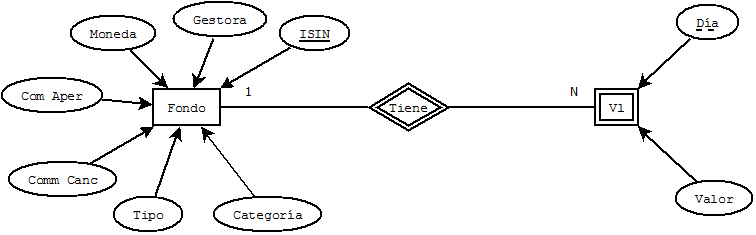
\includegraphics[width=\textwidth]{figuras/ERSimple.png}
	\caption{Diagrama ER inicial}
	\label{fig:erinicial}
\end {figure}

Este modelo está compuesto por una entidad fuerte encargada de guardar la información referente a los fondos y una débil, que presenta una dependencia de identificación con la primera, encargada de guardar los \gls{VL}s de cada fondo. Por tanto, cada fondo puede tener N \gls{VL}s y cada \gls{VL} solo puede pertenecer a un fondo.

\newpage

Este modelo permite almacenar los datos básicos tanto de un fondo como el histórico de sus \gls{VL}s, pero no permite realizar operaciones de compra/venta de participaciones. Para poder realizar operaciones sobre los diferentes fondos es necesario añadir un poco de complejidad al modelo:

\begin{figure}[htbp]
	\centering
	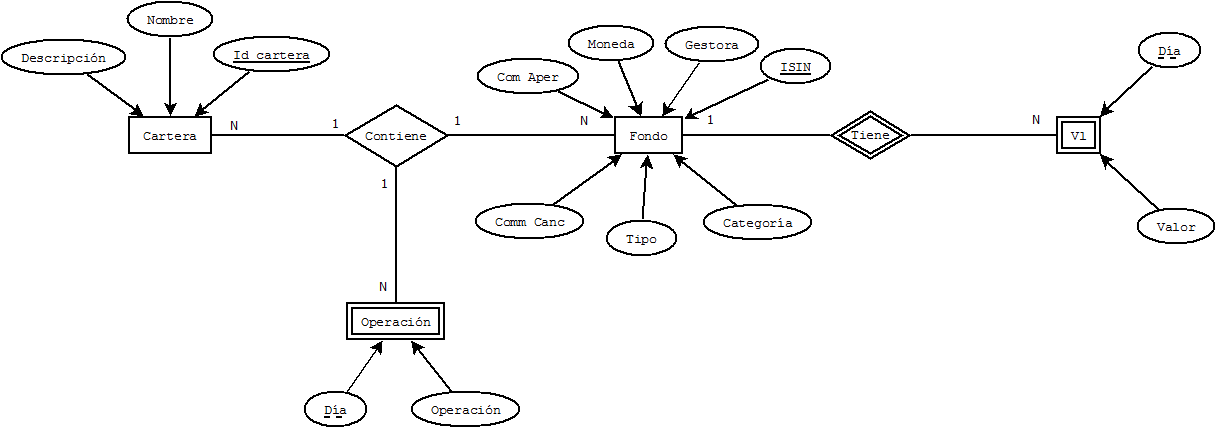
\includegraphics[width=\textwidth]{figuras/ERCompleto.png}
	\caption{Diagrama ER final}
	\label{fig:erfinal}
	\end {figure}

%Diria que esta aproximacion no es correcta, ¿Quizas una entidad debil en el medio en lugar de la relacion "contiene"?


De esta forma incorporamos la posibilidad de tener carteras de fondos y realizar operaciones de compra/venta de participaciones en diferentes fondos pertenecientes a diferentes carteras.\\

Cada fondo de inversión puede pertenecer a varias carteras distintas y cada cartera estará compuesta por varios fondos. Las operaciones sobre ellos solo estarán permitidas si pertenecen a una cartera de inversión, en caso contrario solo se podrá acceder a su histórico de \gls{VL}s.\\

Una vez terminado el diagrama \gls{ER} el siguiente paso es realizar su traducción? al modelo relacional. El resultado es el siguiente:\\

\begin{figure}[htbp]
	\centering
	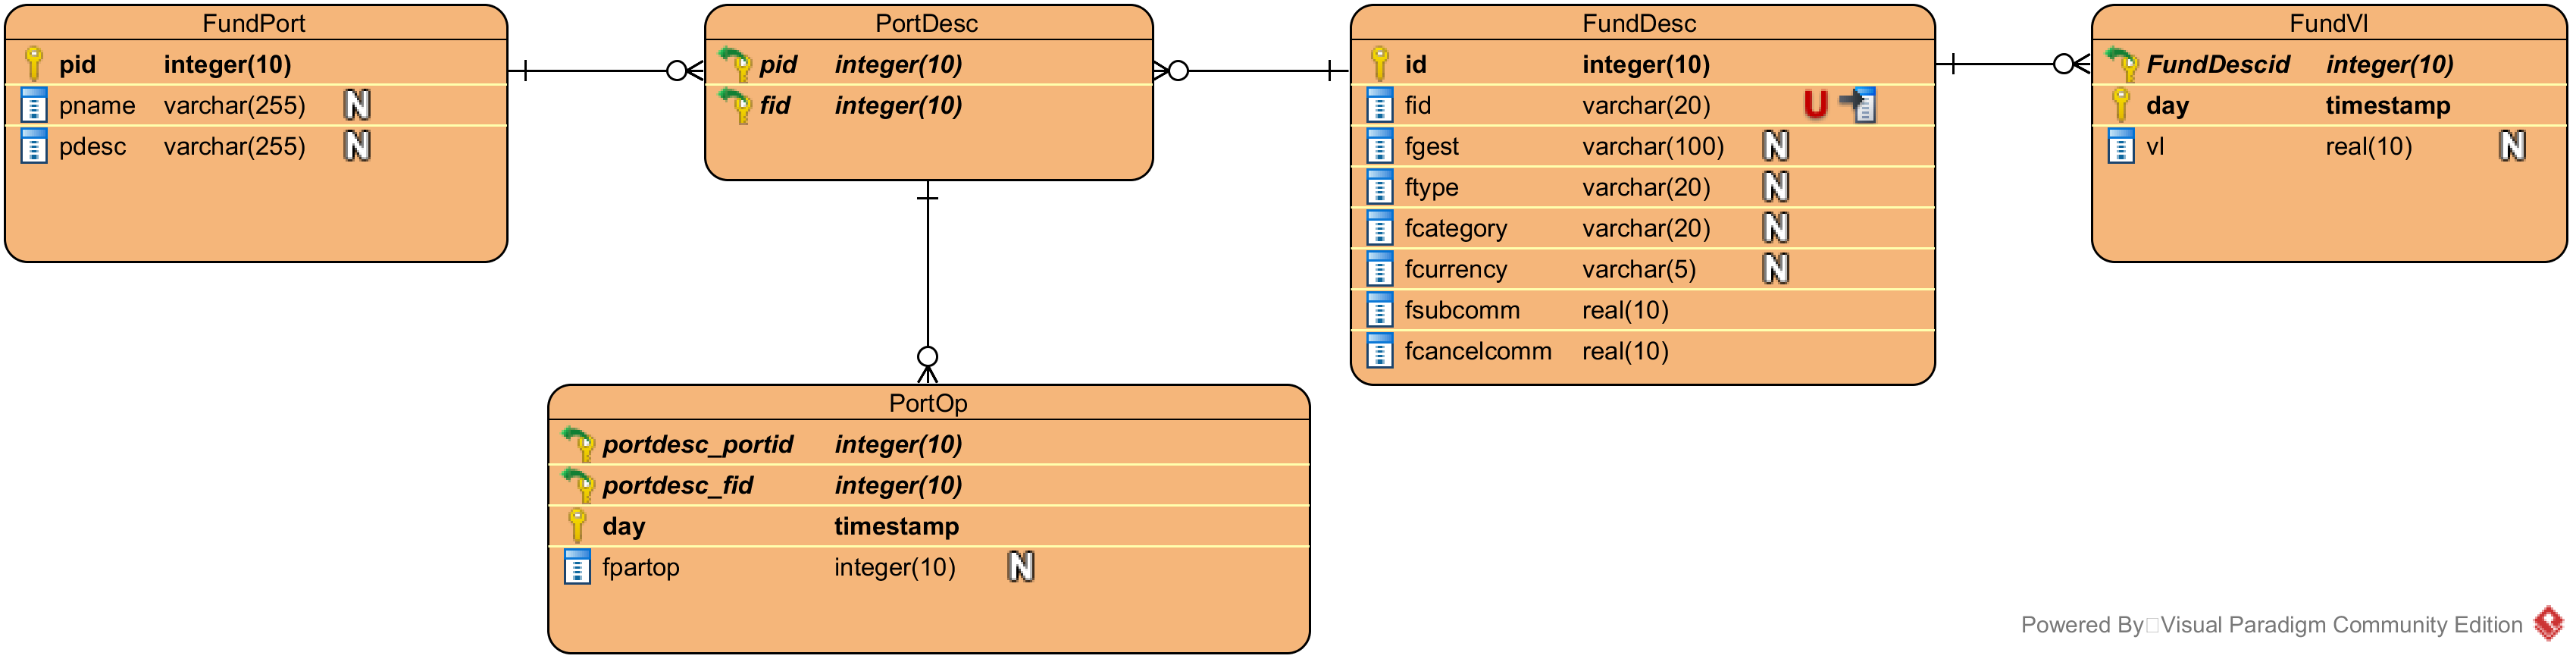
\includegraphics[width=\textwidth]{figuras/DiagramaR.png}
	\caption{Diagrama del modelo relacional(eliminar los nulos)}
	\label{fig:relacional}
	\end {figure}
	
\newpage

\subsection{Implementación de la base de datos mediante Hibernate}

Para implementar la base de datos usando Hibernate, primero debemos modelar las clases Java correspondientes a las tablas del modelo relacional:\\

\begin{figure}[htbp]
	\centering
	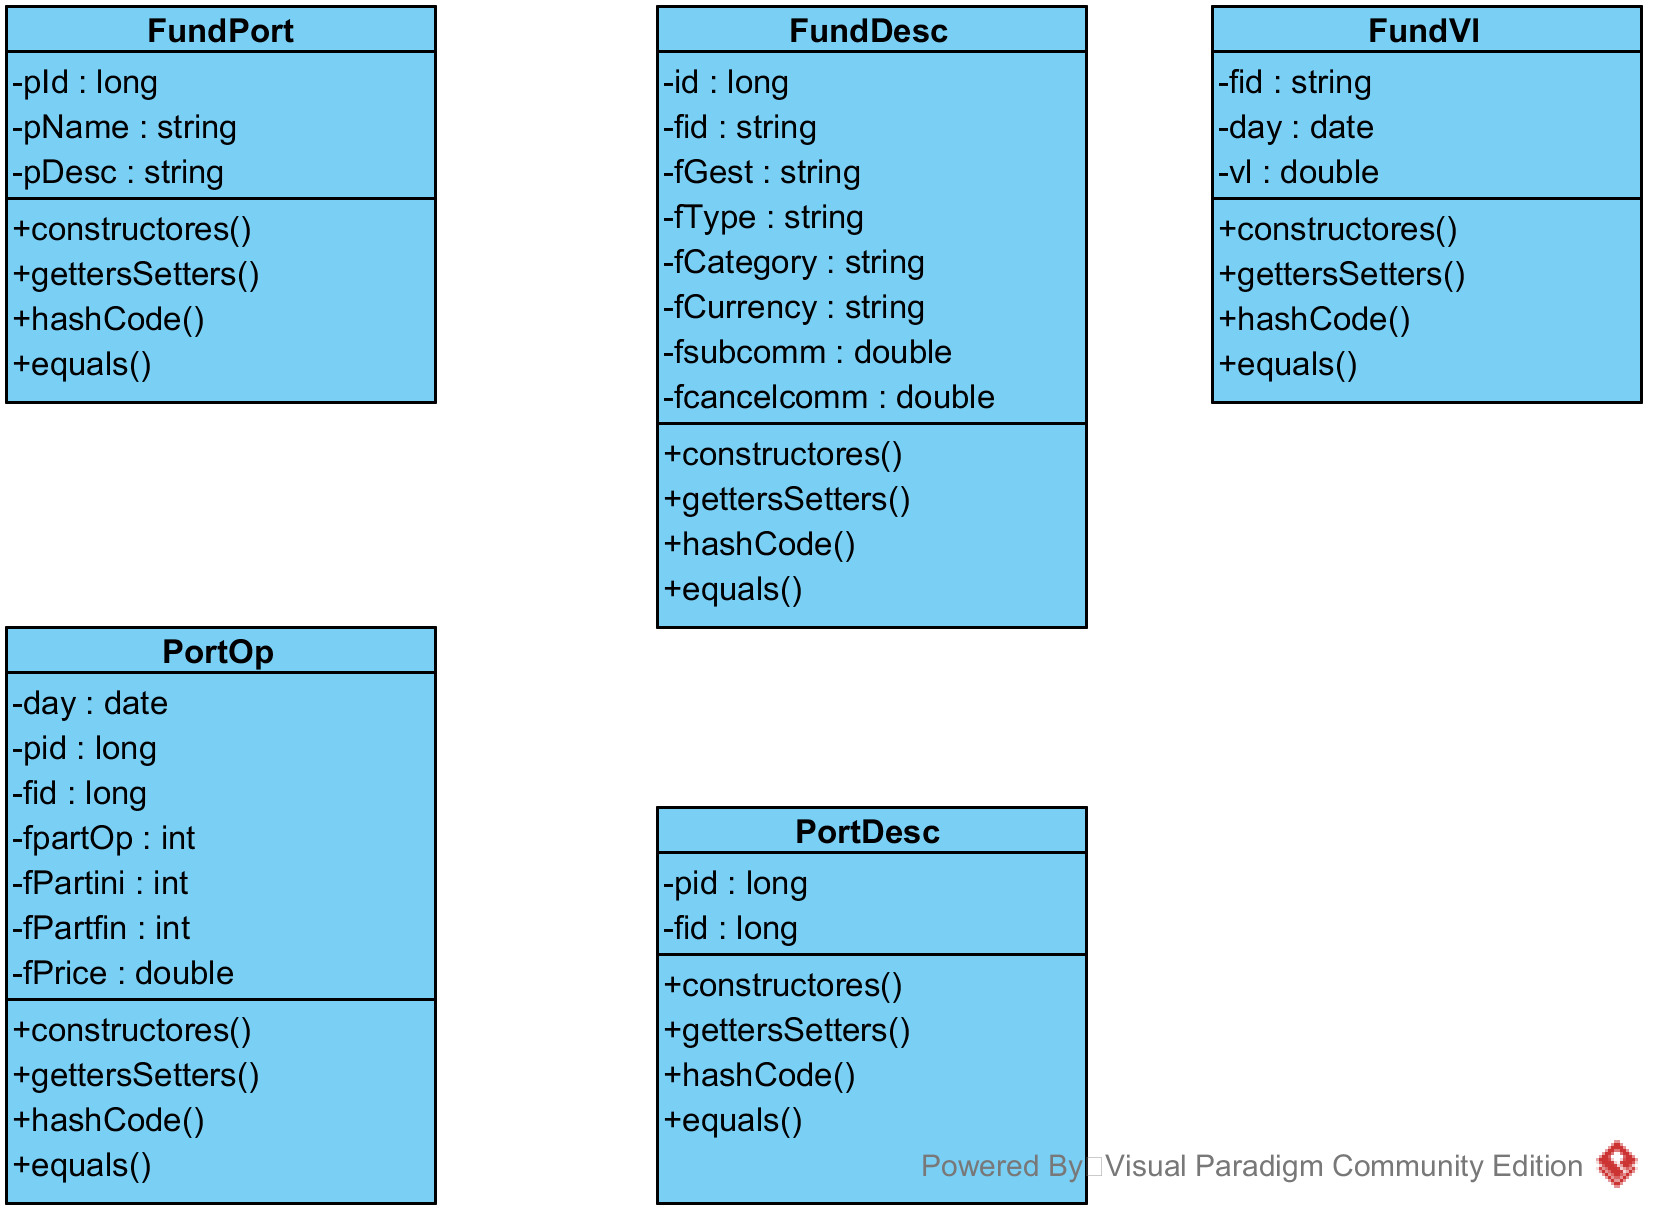
\includegraphics[width=\textwidth]{figuras/Diagrama_clases.png}
	\caption{Diagrama de clases del modelo}
	\label{fig:mclases}
	\end {figure}

Los atributos de FundDesc, \textbf{id} y de FundPort \textbf{pId}, están formados por valores auto generados por la base de datos mediante la estrategia de generación \textit{``GenerationType.IDENTITY"} y actúan como claves primarias de las tablas. En el caso de FunDesc el atributo fId (que se corresponde con el \gls{ISIN} del fondo) es una clave candidata que se guardará en base de datos como un Varchar de longitud 12, indicando a Hibernate que es un valor único y no puede ser nulo. Este atributo podría haberse utilizado como clave primaria de la tabla FundDesc, pero al tratarse de un tipo de dato Varchar que se repetirá, como norma general, más de un millar veces por cada fondo en la tabla FundVl, se ha decidido utilizar un id autogenerado por motivos de rendimiento.\\

Para que Hibernate mapee las relaciones es necesario incluir en cada una de las clases con relación 1:N una lista con los objetos relacionados. Por ejemplo, cada objeto FunDesc tiene, a mayores de los atributos mostrados en el \gls{UML}, uno llamado fundVls y otro llamado portDescs, que contienen una lista de los FundVls y PortDescs relacionados con ese fondo respectivamente.\\

\newpage

En el caso de las relaciones N:1 basta con incluir un atributo del tipo del objeto con el que se relaciona. Por ejemplo, cada objeto FundVl tiene un atributo llamado fundDesc que contiene el fondo al que pertenece ese FundVl. Por este motivo, ha sido necesario modificar la implementación por defecto de los métodos equals y hashcode, para que su uso no provocase una llamada recursiva infinita que causase una excepción por stack overflow.\\


Para poder implementar las clases correspondientes a tablas con claves compuestas en Hibernate, es necesario implementar clases serializables que contengan únicamente los atributos que componen la clave primaria de la tabla. En este caso se han implementado las tres necesarias: % Cambiar por uml?

\begin{itemize}
	\item \textbf{FundVlPk:} Con los atributos fundDesc y day.
	\item \textbf{PortDescPk:} Con los atributos funDescId y fundPortId.
	\item \textbf{PortOpPk:} Con los atributos portDesc y day.
\end{itemize}

En el caso de PortOpPk el atributo portDesc es mapeado en base de datos como el conjunto de las ids del fondo y de la cartera.\\

A continuación, se definen las anotaciones de Hibernate utilizadas para crear la base de datos.

\begin{itemize}
	\item \textbf{@Id:} Indica que el siguiente atributo es la clave primaria de la tabla.
	\item @\textbf{IdClass}: Indica la clase que contiene los atributos que componen la clave primaria de la clase/tabla actual.
	\item  \textbf{@Column:} Indica que el siguiente atributo se modela como una columna en la base de datos.
	\item  \textbf{@Transient:} Indica que el siguiente atributo no se modela como una columna en la base de datos.
	\item \textbf{@GeneratedValue:} Indica que el siguiente atributo es generado automáticamente por la base de datos, utilizando la estrategia asignada.
	\item \textbf{@OneToMany:} Indica que el objeto tiene una relación 1:N con otra tabla.
	\item\textbf{@ManyToOne:} Indica que el objeto tiene una relación N:1 con otra tabla.
	\item\textbf{@JoinColumn:} Indica que el objeto obtiene una columna de otra tabla , normalmente se utiliza junto con la anotación anterior.\\
\end{itemize}

La anotación \textbf{@Transient} se utiliza en la clase PortOp para indicar que los atributos fPartIni, fPartFin y fPrice no se guardan en la base de datos y serán calculados bajo demanda cuando se realice una operación de búsqueda.

\newpage
Las anotaciones @OneToMany y @ManyToOne tienen algunas opciones interesantes:
\begin{itemize}
	\item La opción \textbf{fetch} indica si las listas de objetos relacionados se cargaran bajo demanda (EAGER) o inmediatamente (LAZY).
	\item La opción \textbf{cascade} hace referencia a las acciones que se deben de llevar a cabo tras la eliminación de un objeto, CascadeType.REMOVE indica que se deben eliminar todos los objetos relacionados con el (Por ejemplo si se elimina un FundDesc se eliminan también todos sus FundVls).
	\item La opción \textbf{mappedBy} se utiliza para definir el atributo que mapea la relación entre las tablas.\\
\end{itemize}

 El último paso para crear la base de datos consiste en indicar a Hibernate cuales son las clases que debe mapear en su fichero de configuración \textit{``src/main/resources/hibernate.cfg.xml''}.\\
 
  De esta forma, cuando realicemos la llamada de inicio de sesión \textit{``sessionFactory = new Configuration().configure().buildSessionFactory()"} Hibernate generará las tablas en la base de datos, si no existían previamente.\\
 
  La propiedad \textit{``hbm2ddl.auto"} nos permite controlar el comportamiento de hibernate cuando se inicia la sesión. Podemos, desde eliminar las tablas y volverlas a crear en cada inicio, hasta simplemente actualizarlas si hay cambios.

\newpage

\subsection{Implementación del servicio del modelo}

El servicio del modelo será el encargado de exponer las funcionalidades necesarias para el funcionamiento lógico de la aplicación.\\

Como funcionalidades mínimas necesitamos tener la capacidad de añadir, buscar, actualizar y eliminar elementos de cada una de las tablas de la base de datos, pero a la hora de realizar gráficas es muy interesante, por ejemplo, la posibilidad de obtener los \gls{VL}s y las operaciones sobre un fondo en un rango de fechas determinado, por lo que el servicio consta de los siguientes métodos:\\

\begin{figure}[htbp]
	\centering
	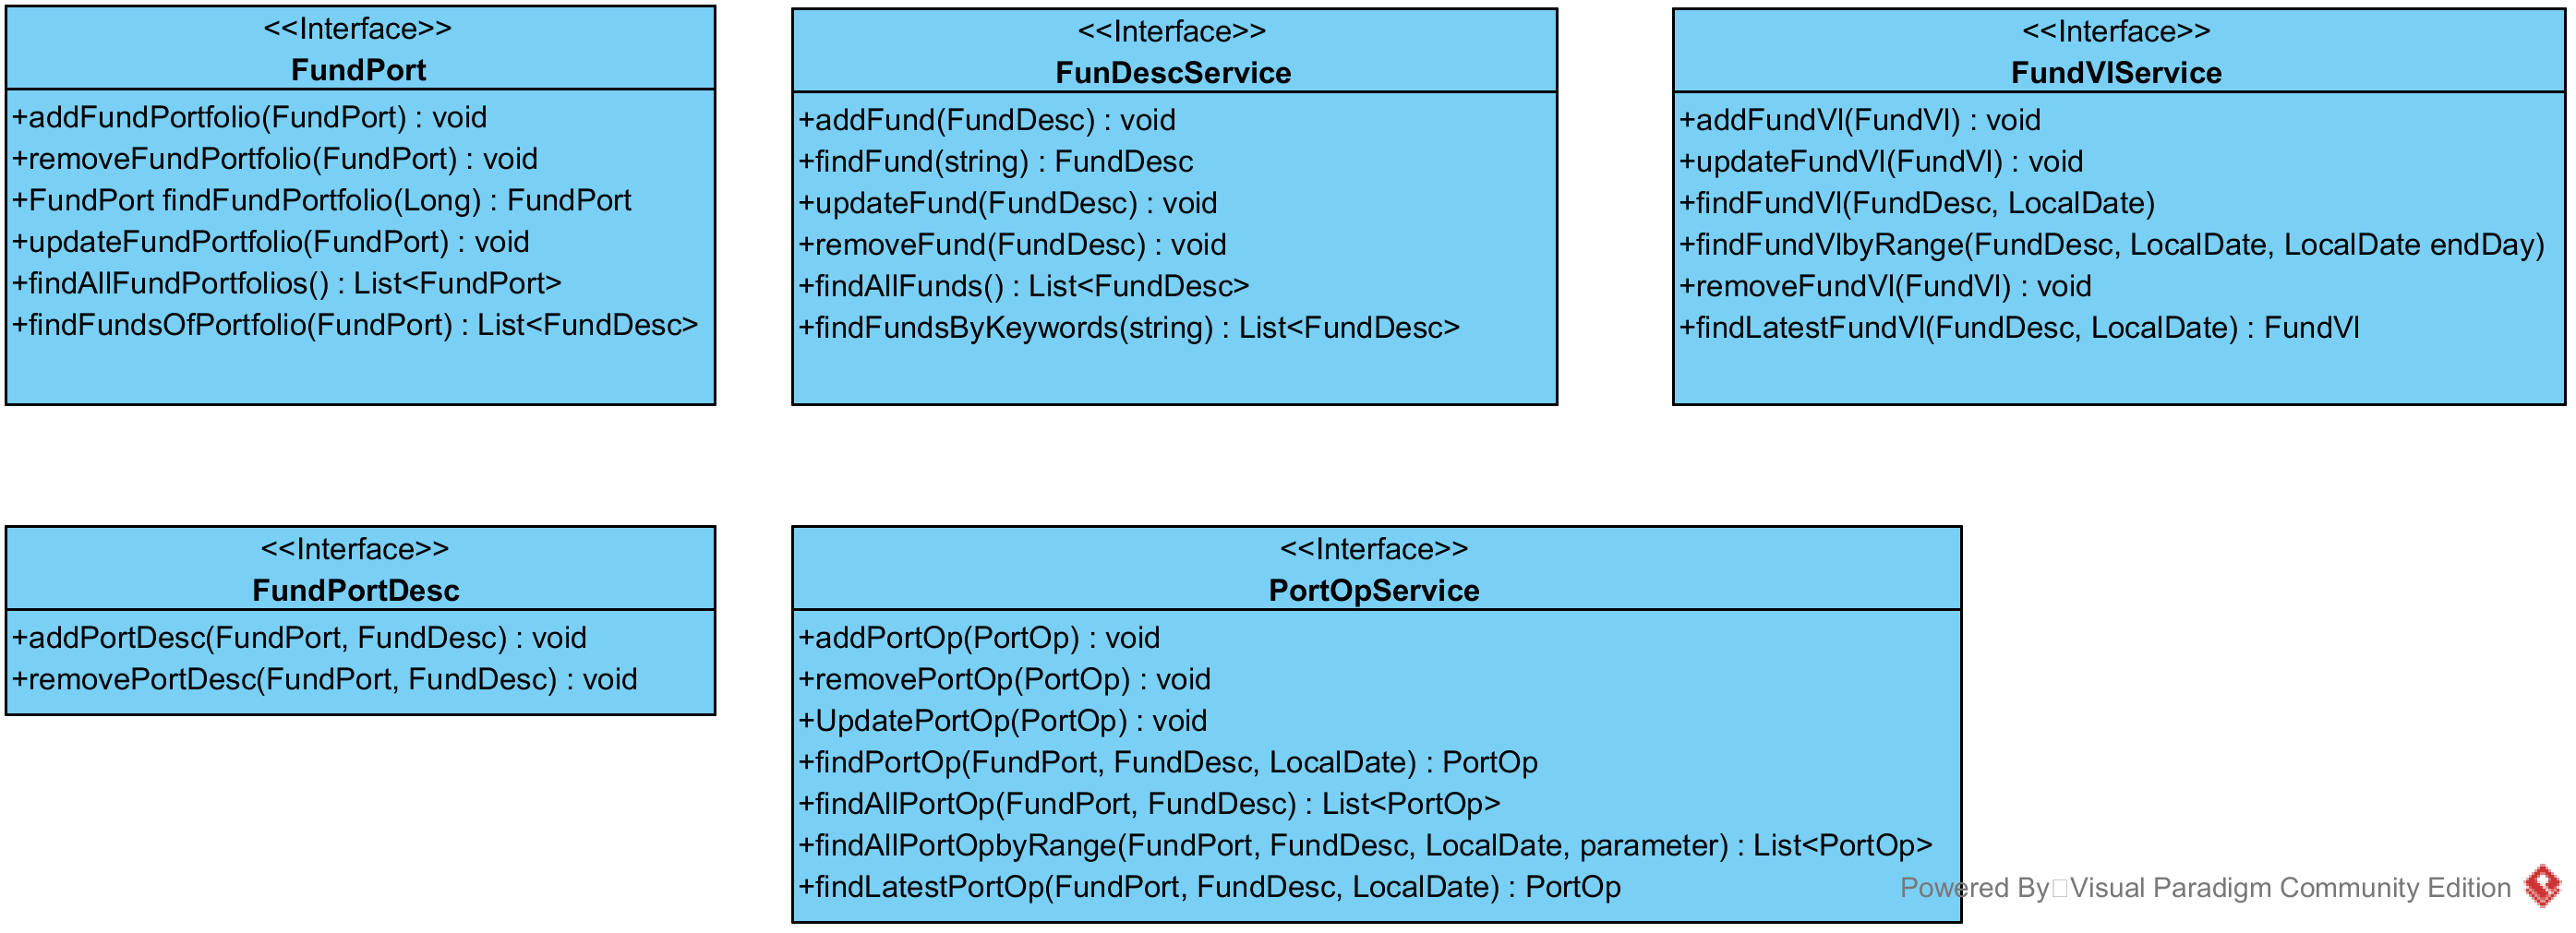
\includegraphics[width=\textwidth]{figuras/Diagrama_Modelo.png}
	\caption{Diagrama del servicio}
	\label{fig:relacional}
	\end {figure}

Aunque en este diagrama existe una interfaz del servicio para cada clase, en la implementación se han agrupado todos en una única interfaz denominada \textbf{FundService}.\\

Cada uno de los métodos del servicio lanza una \textbf{RunTimeException} si se produce algun error a la hora de conectarse a la base de datos. A mayores, se han implementado dos excepciones más:

\begin{itemize}
	\item \textbf{InputValidationException:} Salta cuando los datos introducidos por el usuario no son correctos.
	\item \textbf{InstanceNotFoundException:} Salta cuando no se puede encontrar el objeto solicitado en la base de datos.
\end{itemize}


Para llevar a cabo la validación de los datos de entrada se ha incorporado un validador: \\

uml del validador\\

\newpage

Existen una serie de métodos en el servicio que utilizan este validador para asegurar que los datos introducidos son correctos:

\begin{itemize}
	\item \textbf{validateFundVl:} se encarga de validar que el campo vl del FundVl es mayor o igual que cero.
	\item \textbf{validateFund:} se encarga de validar que el \gls{ISIN} del fondo es correcto y llama a su vez a validateFundVl para validar cada uno de sus FundVl.
	\item \textbf{validateFundPort:} se encarga de validar que el nombre de la cartera de fondos no sea un string vacío.
	\item \textbf{validatePortOp:} se encarga de validar que la operación añadida, eliminada o actualizada no deje en ningún momento a la base de datos con un total de participaciones negativo.
\end{itemize}

Ahora analizaremos cada método por separado:

\begin{itemize}
	\item FundDesc
						 \begin{itemize}
							\item \textbf{addFund:} Añade un FundDesc y toda su lista de FundVLs a la base de datos. La forma más común de representación de un fondo es mediante un fichero excel (.xls) que contenga un conjunto de pares día-\gls{VL}, en un futuro la aplicación permitirá importar los \gls{VL}s a partir de estos ficheros, por lo que se podrán guardar en la base de datos simplemente llamando a esta operación.
							\item \textbf{findFund:} Devuelve el FundDesc a partir de su \gls{ISIN}. A pesar de que la clave primaria de la tabla sea la clave subrogada \textit{``id"}, es más natural buscar un fondo en concreto por su \gls{ISIN}.
							\item \textbf{updateFund:} Actualiza los campos de un FundDesc.
							\item \textbf{removeFund:} Elimina un FundDesc y toda su lista de FundVls de la base de datos.
							\item \textbf{findAllFunds:} Obtiene todos los FundDesc de la base de datos.
							\item \textbf{findFundsByKeywords:} Obtiene los fundDesc que coinciden con una serie de caracteres en alguno de sus campos. Esta función es útil a la hora de buscar varios fondos de un mismo tipo, moneda o gestora, por ejemplo.
				 		 \end{itemize}
	\item FundPort
						\begin{itemize}
							\item \textbf{addFundPortfolio:} Añade una cartera de fondos.
							\item \textbf{removeFundPortfolio:} Elimina una cartera de fondos.
							\item \textbf{findFundPortfolio:} Obtiene una cartera de fondos a partir de su Id.
							\item \textbf{updateFundPortfolio:} Actualiza los campos de una cartera de fondos.
							\item \textbf{findAllFundPortfolios:} Obtiene todas las carteras de la base de datos.
							\item \textbf{findFundsOfPortfolio:} Obtiene todos los fondos de una cartera.
						\end{itemize}
					\newpage
	\item FundVl
						\begin{itemize}
							\item\textbf{addFundVl:} Añade un unico FundVl a un fondo en un día concreto.
							\item\textbf{removeFundVl:} Elimina una fila de la tabla vl de un fondo en un dia concreto.
							\item \textbf{findFundVl:}Obtiene el FundVl de un fondo en un dia concreto.
							\item \textbf{updateFundVl:} Actualiza un unico FundVl de un fondo en un día concreto.
							\item \textbf{findFundVlByRange:} Obtiene los Vl de un fondo dado en el intervalo de tiempo deseado.
							\item \textbf{findLatestFundVl:} Obtiene el FundVl del día mas próximo a uno dado (Se comporta exactamente igual a findFundVl si existe un valor vl en ese día). Esta función se utiliza para calcular el valor monetario de una operación. Cuando no se disponga del \gls{VL} de un fondo el dia de la operación, se utilizará en su lugar el valor del día anterior más cercano.
						\end{itemize}
				
	\item PortDesc
						\begin{itemize}
							\item\textbf{addPortDesc:} Añade un fondo a una cartera.
							\item\textbf{removePortDesc:} Elimina un fondo de una cartera.
						\end{itemize}
	\item PortOp
						\begin{itemize}
							\item\textbf{addPortOp:} Añade una operacion (Con participaciones como unidad) sobre un fondo en una cartera en un día determinado.
							\item\textbf{removePortOp:} Elimina una operacion realizada sobre un fondo en una cartera en una fecha.
							\item \textbf{findPortOp:} Obtiene una operacion sobre un fondo en una cartera en un día determinado.
							\item \textbf{updatePortOp:} Actualiza un PortOp (Con participaciones como unidad) sobre un fondo en una cartera en un día determinado.
							\item \textbf{findAllPortOp:} Devuelve todas las operaciones realizadas sobre un fondo en una cartera.
							\item \textbf{findPortOpByRange:} Devuelve todas las operaciones realizadas sobre un fondo en una cartera entre dos fechas.
							\item \textbf{findLatestPortOp:} Obtiene el la operacion sobre un fondo en una cartera del dia mas proximo a un dia dado (Se comporta exactamente igual a findPortOp si existe un PortOp en ese dia). Esta función se utiliza para conocer cual ha sido la operación mas reciente sobre un fondo, lo que permite ver las participaciones que tenemos invertidas en el.\\
						\end{itemize}
	
\end{itemize}

Como se ha comentado anteriormente, los campos de los objetos PortOp:  fPartIni, fPartFin y fPrice se calculan bajo demanda en los métodos de búsqueda findPortOp, findAllPortOp, findPortOpByRange y findLatestPortOp. La operación encargada de calcularlos es calculatePortOp.\\

\newpage

El método \textbf{calculatePortOp} revisa todas las operaciones anteriores y obtiene el numero de participaciones inicial y final, además del precio de la operación, utilizando para ello el vl más próximo y teniendo en cuenta las comisiones de apertura y cancelación del fondo.\\

Se utiliza esta operación en lugar de almacenar directamente los valores de los campos en la base de datos debido a que si se guardasen, cada inserción, actualización o borrado de una operación, implicaría actualizar todos los valores de las operaciones siguientes, además de estar guardando información redundante que se puede calcular directamente con los datos que ya se encuentran en la base de datos.



\newpage
\part{Bibliografía}

\begin{thebibliography}{10}
	
	\bibitem[CNMV]{}
	\newblock {\textit{Comisión Nacional del Mercado de Valores}.}
	\newline
	\href{https://www.cnmv.es/}{https://www.cnmv.es/}
	
	\bibitem[Rankia]{}
	\newblock {\textit{Todo lo que hay que saber de Fondos de inversión en un único artículo}.}
	\newline
	\href{http://www.rankia.com/blog/fondos-inversion/3208096-todo-que-hay-saber-fondos-inversion-unico-articulo}{http://www.rankia.com/blog/fondos-inversion/3208096-todo-que-hay-saber-fondos-inversion-unico-articulo}
	
	\bibitem[Rankia]{}
	\newblock {\textit{¿Qué es un fondo de inversión y cómo funciona?}.}
	\newline
	\href{http://www.rankia.com/blog/fondos-inversion/952310-que-fondo-inversion-como-funciona}{http://www.rankia.com/blog/fondos-inversion/952310-que-fondo-inversion-como-funciona}
	
	\bibitem[Wikipedia]{}
	\newblock {\textit{Proceso Unificado de Desarrollo Software}.}
	\newline
	\href{https://es.wikipedia.org/wiki/Proceso\_unificado}{https://es.wikipedia.org/wiki/Proceso\_unificado}
	
\end{thebibliography}
\newpage
\setglossarystyle{tree}
\printglossary[type=\acronymtype]

\end{document}